% !TeX root = RJwrapper.tex
\title{hcinfer: An R Package for Heteroskedasticity-Consistent Inference in Linear Regression}


\author{by Pedro Rafael D. Marinho, Francisco Cribari-Neto, and Marina Oliveira Cunha}

\maketitle

\abstract{%
Ordinary least squares regression is a standard tool in applied statistics, but its usual standard errors assume constant error variance. When this assumption fails, tests and confidence intervals based on the conventional covariance matrix can be misleading, even though the coefficient estimates remain unbiased. Heteroskedasticity-consistent covariance estimators correct this problem without a parametric model for the error variances, but different estimators can produce substantially different inferences, especially when high-leverage observations are present. The hcinfer package for R provides a focused workflow for heteroskedasticity-consistent inference in linear models fitted with lm. It computes the HC0 through HC5m estimators together with HCbeta, a leverage-sensitive estimator proposed by the package authors that adjusts the residual weights through a beta distribution fitted to the leverage values. Covariance estimation is coupled with coefficient-level normal Wald tests, confidence intervals, leverage diagnostics, adjustment-factor inspection, and graphical reporting behind a small and consistent interface that reuses the standard R generics. Two complementary tools broaden the same workflow: a pairs bootstrap that supplies assumption-free empirical standard errors and intervals as a reference for the analytic estimators, and feasible generalized least squares under multiplicative heteroskedasticity, fitted by Harvey's two-step method or by Gaussian maximum likelihood with information criteria. An analysis of public school expenditure data illustrates the package and shows how the choice of covariance estimator can change the substantive conclusion, while the default HCbeta estimator avoids the very large adjustment factors that some high-leverage estimators produce.
}

\section{Introduction}\label{introduction}

Linear regression models fitted by ordinary least squares are widely used in empirical research because of their interpretable parameters, well-established diagnostic tools, and stable implementation in statistical software. Statistical inference in such models, however, depends critically on the covariance matrix used for the coefficient estimates. The conventional covariance estimator is derived under the assumption of homoskedastic errors. When error variances differ across observations, standard errors based on this assumption may distort hypothesis tests and confidence intervals, even though the coefficient estimates remain unbiased under the usual exogeneity conditions.

Heteroskedasticity is often a structural feature of applied data rather than a mere diagnostic irregularity. In cross-sectional economic, educational, and social applications, responses associated with larger, wealthier, or more heterogeneous units frequently display greater conditional variability. Firm-level outcomes may scale with size, regional indicators may aggregate units with very different characteristics, and survey or administrative data may combine measurements with unequal precision. In such settings, reliable inference requires covariance estimators that remain valid without restrictive variance assumptions.

Heteroskedasticity-consistent (HC) covariance matrix estimators provide a nonparametric correction to this problem. The seminal estimator of \citet{White1980} replaces the scalar error variance in the ordinary least squares covariance matrix with a diagonal matrix formed by squared residuals. Subsequent proposals refine this construction through finite-sample and leverage-based adjustment factors. These include HC1 \citep{Hinkley1977}, HC2 \citep{MacKinnonWhite1985}, HC3 \citep{MacKinnonWhite1985, DavidsonMacKinnon1993}, HC4 \citep{CribariNeto2004}, HC4m \citep{CribariNetoDaSilva2011}, HC5 \citep{CribariNetoSouzaVasconcellos2007}, HC5m \citep{Li2016}, and the more recent \(\text{HC}_\beta\) \citep{Cunha+Cribari+Marinho_2026_arXiv}. Although all of these estimators converge to the same asymptotic sandwich form, their finite-sample behavior can differ substantially, which is precisely the regime where the choice among them affects substantive conclusions.

The \CRANpkg{hcinfer} package for R implements this family of HC estimators for linear models fitted with \texttt{lm()} \citep{RCoreTeam2026, MarinhoHcinfer2026}. Although robust covariance estimation is already well established in R through the \CRANpkg{sandwich} package \citep{Zeileis2004, Zeileis2006}, which provides a broad framework for HC and HAC estimation, \CRANpkg{hcinfer} has a more specialized and complementary purpose. It focuses exclusively on HC inference for linear regression models and integrates covariance estimation, coefficient-level normal Wald tests, confidence intervals, leverage diagnostics, adjustment-factor inspection, and graphical reporting into a unified framework. Beyond covariance estimation, the package also provides a pairs bootstrap that yields assumption-free empirical standard errors as a reference for the analytic estimators, and feasible generalized least squares under a multiplicative variance model, fitted either by Harvey's two-step procedure or by Gaussian maximum likelihood. Its default estimator is \(\text{HC}_\beta\), reflecting the package authors' view that a leverage-sensitive correction is a reasonable starting point for routine inference in modest samples.

This article presents \texttt{hcinfer} as a statistical software contribution for heteroskedasticity-robust inference in linear regression. The emphasis is on the package interface, implementation, and practical use, while the mathematical development is included only to define the quantities computed and to clarify the relationships among the available estimators. Section 2 reviews HC covariance estimators and normal Wald inference, and introduces the pairs bootstrap and feasible generalized least squares under multiplicative heteroskedasticity. Section 3 introduces the package interface. Section 4 discusses implementation details. Section 5 presents an empirical illustration and an estimator comparison. Section 6 documents software availability and reproducibility, and Section 7 summarizes the contribution.

\section{Statistical background}\label{statistical-background}

Robust covariance estimation starts from the usual ordinary least squares model and changes the estimator of its covariance matrix. This section defines the model, residuals, leverage values, and adjustment factors used by every method implemented in \CRANpkg{hcinfer}. Consider the linear regression model
\[
\mathbf{y} = X\boldsymbol{\beta} + \mathbf{e},
\]
where \(\mathbf{y}\) is an \(n \times 1\) response vector, \(X\) is an \(n \times p\) full-rank design matrix with \(p < n\), \(\boldsymbol{\beta}\) is a \(p \times 1\) parameter vector, and \(\mathbf{e}\) is an \(n \times 1\) error vector. For \(t = 1, \ldots, n\), \(\mathbb{E}(e_t)=0\) and \(\operatorname{Var}(e_t)=\sigma_t^2 < \infty\). The ordinary least squares estimator of \(\boldsymbol{\beta}\) is
\[
\hat{\boldsymbol{\beta}} = (X'X)^{-1}X'\mathbf{y},
\]
and \(\hat{e}_t = y_t - \mathbf{x}_t'\hat{\boldsymbol{\beta}}\) denotes the ordinary least squares residual for observation \(t\).

The covariance matrix of \(\hat{\boldsymbol{\beta}}\) is
\[
\Psi = (X'X)^{-1}X'\Omega X(X'X)^{-1},
\]
where \(\Omega = \operatorname{diag}(\sigma_1^2,\ldots,\sigma_n^2)\). HC estimators of \(\Psi\) replace \(\Omega\) with
\[
\widehat{\Omega} = \operatorname{diag}(\hat{e}_1^2 g_1,\ldots,\hat{e}_n^2 g_n),
\]
yielding the sandwich estimator
\begin{equation}
\widehat{\Psi}_{HC} = (X'X)^{-1}X'\widehat\Omega X(X'X)^{-1}.
\label{eq:sandwich}
\end{equation}
The estimators differ only through the adjustment factors \(g_t\), which is why the sandwich form in Equation \eqref{eq:sandwich} can host a whole family of HC estimators behind a single template.
The diagonal entries of \(\widehat{\Omega}\) therefore combine squared residuals with method-specific corrections before the outer matrices map them to coefficient covariances.

These adjustment factors typically depend on the leverage of each observation. The hat matrix is
\[
H = X(X'X)^{-1}X',
\]
and its \(t\)th diagonal element is denoted by \(h_t\). The quantity \(h_t\) measures the leverage of observation \(t\), and the average leverage is \(\bar{h} = p/n\). Because \(h_t\) identifies observations that exert unusual influence on the fitted values, it is the natural quantity through which a leverage-sensitive correction can be calibrated within the sandwich framework.

For HC0, \(g_t = 1\). HC1 uses \(g_t = n/(n-p)\). HC2 uses \(g_t = (1-h_t)^{-1}\), and HC3 uses \(g_t = (1-h_t)^{-2}\). The HC4 and HC4m estimators take the form \(g_t=(1-h_t)^{-\delta_t}\), with
\[
\delta_t = \min\left(4, \frac{h_t}{\bar{h}}\right)
\]
for HC4 and
\[
\delta_t = \min\left(1, \frac{h_t}{\bar{h}}\right)
+ \min\left(1.5, \frac{h_t}{\bar{h}}\right)
\]
for HC4m. These piecewise definitions let the exponent grow with leverage up to a cap, so that the correction strengthens for high-leverage points while remaining bounded.

HC5 and HC5m extend these leverage-based adjustments to accommodate more extreme leverage patterns. Let \(h_{\max} = \max(h_1,\ldots,h_n)\). HC5 uses \(g_t=(1-h_t)^{-\delta_t}\), where
\[
\delta_t = \min\left(
\frac{h_t}{\bar{h}},
\max\left(4, k\frac{h_{\max}}{\bar{h}}\right)
\right),
\qquad k = 0.7.
\]
By contrast with HC4, the cap of HC5 itself grows with the most extreme leverage value, so the correction can track designs in which one observation is far more influential than the rest. HC5m combines the adjustment structures of HC4m and HC5:
\[
\delta_t
=
k_1\min\left(\gamma_1, \frac{h_t}{\bar{h}}\right)
+
k_2\min\left(\gamma_2, \frac{h_t}{\bar{h}}\right)
+
k_3\min\left(
\frac{h_t}{\bar{h}},
\max\left(4, k\frac{h_{\max}}{\bar{h}}\right)
\right),
\]
with defaults \(k=0.7\), \(k_1=1\), \(k_2=0\), \(k_3=1\), \(\gamma_1=1\), and \(\gamma_2=1.5\), and \(g_t=(1-h_t)^{-\delta_t}\). With these defaults, HC5m combines the first capped HC4m component with the HC5 component and omits the second capped component.

\(\text{HC}_\beta\) uses the leverage complement \(u_t = 1 - h_t\) and its truncated version \(w_t = \max\left(0.01, \min(u_t, 0.99)\right)\). The beta shape parameters, \(a\) and \(b\), are estimated by the method of moments from \(w_t\), then shrunk toward the uniform case \(a = b = 1\):
\begin{equation}
\zeta = \frac{n}{n+50}, \quad
\tilde{a} = (1-\zeta) + \zeta\hat{a}, \quad
\tilde{b} = (1-\zeta) + \zeta\hat{b},
\label{eq:shrinkage}
\end{equation}
where \(\hat{a}\) and \(\hat{b}\) are the method-of-moments estimators of the beta shape parameters. The shrinkage in Equation \eqref{eq:shrinkage} regularizes the fitted beta distribution toward the uniform distribution, which keeps the adjustment stable when the empirical leverage distribution is sparse or skewed in a small sample. The \(\text{HC}_\beta\) adjustment factor is
\[
g_t =
\frac{n}{n-p}
\left(
\frac{1}{F_B(w_t;\tilde{a},\tilde{b})}
\right)^{c_1/n^{c_2}},
\qquad c_1=7, \quad c_2=0.75,
\]
where \(F_B(\cdot;\tilde{a},\tilde{b})\) denotes the cumulative distribution function of a beta distribution with shape parameters \(\tilde{a}\) and \(\tilde{b}\). The beta CDF provides a smooth generalization of the uniform CDF, but its use here does not assume that \(u_t\) follows a beta distribution. When \(c_1=0\), the exponent \(c_1/n^{c_2}\) is zero and the bracketed factor equals one, so \(\text{HC}_\beta\) reduces exactly to HC1 for any finite positive fitted shape parameters. As \(n\) grows, \(c_1/n^{c_2}\to0\) and \(n/(n-p)\to1\), so \(g_t\to1\) and the HC0 structure is recovered asymptotically. The correction is designed to adapt to the leverage structure rather than imposing a fixed or piecewise power of \((1-h_t)\).

For a coefficient \(\beta_j\), \texttt{hcinfer} tests
\[
\mathcal{H}_0 \colon \beta_j = \beta_j^{(0)}, \qquad j = 1,\ldots,p,
\]
using
\[
z_j =
\frac{\hat\beta_j - \beta_j^{(0)}}
{\sqrt{[\widehat\Psi_{HC}]_{jj}}},
\]
where \([\widehat\Psi_{HC}]_{jj}\) is the \(j\)th diagonal element of \(\widehat{\Psi}_{HC}\). Under \(\mathcal{H}_0\), \(z_j\) is asymptotically standard normal, so inference is based on approximate normal critical values. As a consequence, the finite-sample rejection rates may differ from the nominal significance level, particularly in small samples or in designs with influential high-leverage observations. The corresponding \((1-\alpha)\) confidence interval is
\[
\hat{\beta}_j
\pm
z_{1-\alpha/2}
\sqrt{[\widehat{\Psi}_{HC}]_{jj}},
\]
and it contains \(\beta_j\) with probability that approaches \(1-\alpha\) when \(n \to \infty\).

\subsection{Pairs bootstrap as an empirical reference}\label{pairs-bootstrap-as-an-empirical-reference}

Analytic HC standard errors can also be checked against a resampling reference. The \texttt{boot\_pairs()} function computes the pairs, or case, bootstrap for the ordinary least squares coefficients \citep{DavisonHinkley1997, EfronTibshirani1993}. Each of \(B\) replicates draws \(n\) observation indices with replacement from \(\{1,\ldots,n\}\), refits ordinary least squares on the resampled pairs \((y_i,\mathbf{x}_i)\), and stores the replicate estimate \(\hat{\boldsymbol{\beta}}^{*}_{(r)}\). The bootstrap standard error of coefficient \(j\) is the sample standard deviation of \(\hat\beta^{*}_{1,j},\ldots,\hat\beta^{*}_{B,j}\). Because it resamples whole observations, the pairs bootstrap makes no assumption about the form of the error variance, so it is an assumption-free empirical companion to the analytic estimators rather than a substitute for them.

Three interval types are available. Writing \(q_\alpha\) for the empirical \(\alpha\) quantile of the replicates, \(\hat\beta_j\) for the original estimate, \(s^{*}_j\) for the bootstrap standard error, and \(\alpha=1-\texttt{level}\), the percentile interval is \([q_{\alpha/2},\,q_{1-\alpha/2}]\), the basic (reverse percentile) interval is \([2\hat\beta_j-q_{1-\alpha/2},\,2\hat\beta_j-q_{\alpha/2}]\), and the normal interval is \(\hat\beta_j\pm z_{1-\alpha/2}\,s^{*}_j\). The resampling is reproducible through a \texttt{seed} argument, and, because all indices are drawn once in the main process, the result is identical whether the replicate fits run sequentially or in parallel. Resamples that turn out rank deficient are dropped with a warning, and the summaries use the remaining replicates.

\subsection{Feasible generalized least squares under multiplicative heteroskedasticity}\label{feasible-generalized-least-squares-under-multiplicative-heteroskedasticity}

The HC estimators robustify the covariance matrix while leaving the ordinary least squares coefficients unchanged. A complementary strategy models the error variance explicitly and reweights the fit. When the conditional variance can be described by observed regressors, \CRANpkg{hcinfer} provides feasible generalized least squares under a multiplicative variance model through \texttt{gls\_mult()}. The mean model is \(\mathbf{y}=X\boldsymbol{\beta}+\mathbf{e}\) with \(e_t=\sigma_t\varepsilon_t\) and \(\varepsilon_t\stackrel{\mathrm{iid}}{\sim}N(0,1)\), and the variance is
\[
\sigma_t^2=\exp(\eta_t),\qquad \eta_t=\mathbf{z}_t'\boldsymbol{\gamma},
\]
where \(\mathbf{z}_t\) is the \(t\)th row of an \(n\times q\) full-rank dispersion matrix \(Z\) that contains an intercept, and \(\boldsymbol{\gamma}\) is the log-variance coefficient vector. The exponential link keeps the fitted variances positive for every \(\boldsymbol{\gamma}\), and \(\exp(\eta_t/2)\) is the conditional standard deviation in the units of the response. Unlike the HC estimators, this route places a testable assumption on the variance, so it suits settings in which the analyst is willing to model the heteroskedasticity rather than only guard against it.

The two-step estimator, selected with \texttt{estimator\ =\ "two\_step"}, follows \citet{Harvey1976}. It regresses \(\log(\hat e_t^2)\) on \(Z\) to obtain a preliminary \(\tilde{\boldsymbol{\gamma}}\) and corrects the dispersion intercept by the additive constant \(c=-\psi(1/2)-\log 2\approx 1.2704\), where \(\psi\) is the digamma function, because \(\mathbb{E}\{\log(\varepsilon_t^2)\}=-c\) under normality. The corrected coefficients give inverse-variance weights \(\hat w_t=\exp(-\mathbf{z}_t'\hat{\boldsymbol{\gamma}})\) and the feasible generalized least squares estimator
\[
\hat{\boldsymbol{\beta}}_{\mathrm{GLS}}=(X'\widehat W X)^{-1}X'\widehat W\mathbf{y},
\qquad \widehat W=\operatorname{diag}(\hat w_1,\ldots,\hat w_n),
\]
whose reported model-based covariance \((X'\widehat W X)^{-1}\) treats the estimated weights as known, the convention of \citet{CribariNetoPereira2019}. The asymptotic covariance of the auxiliary regression is \((\pi^2/2)(Z'Z)^{-1}\), since \(\pi^2/2\) is the variance of \(\log(\chi^2_1)\).

The default estimator, \texttt{estimator\ =\ "ml"}, maximizes the Gaussian log-likelihood of the same specification,
\[
\ell(\boldsymbol{\beta},\boldsymbol{\gamma})=
-\frac{n}{2}\log(2\pi)
-\frac{1}{2}\sum_{t=1}^{n}\mathbf{z}_t'\boldsymbol{\gamma}
-\frac{1}{2}\sum_{t=1}^{n}\exp(-\mathbf{z}_t'\boldsymbol{\gamma})(y_t-\mathbf{x}_t'\boldsymbol{\beta})^2,
\]
profiling \(\boldsymbol{\beta}\) out by weighted least squares at each trial \(\boldsymbol{\gamma}\) so that the optimizer searches only the \(q\)-dimensional dispersion space. The expected information is block diagonal, with \(\mathcal{I}_{\beta\beta}=X'WX\) and \(\mathcal{I}_{\gamma\gamma}=\tfrac{1}{2}Z'Z\), which yields the reported dispersion covariance \(2(Z'Z)^{-1}\) and the mean covariance \((X'\widehat W X)^{-1}\). Because a maximum likelihood fit carries a genuine log-likelihood with \(p+q\) degrees of freedom, \texttt{logLik()}, and hence \texttt{AIC()} and \texttt{BIC()}, compare competing variance specifications directly; with an intercept-only dispersion model the fit reduces to the homoskedastic Gaussian linear model. The reported covariance is model based and therefore relies on correct specification of the variance model, so \texttt{gls\_mult()} complements rather than replaces the HC estimators, which remain the appropriate choice when no variance model is assumed.

\section{Overview of the hcinfer package}\label{overview-of-the-hcinfer-package}

The package is organized around two main entry points that follow a common interface. The covariance function, \texttt{vcov\_hc(object,\ type,\ ...)}, computes a heteroskedasticity-consistent covariance estimator and returns an S3 object containing the covariance matrix, residuals, leverage values, HC adjustment factors, method parameters, coefficient names, model metadata, and dimension information. The inference function, \texttt{hcinfer(object,\ type,\ alpha,\ null,\ ...)}, builds on \texttt{vcov\_hc()} and augments its output with coefficient-level test statistics, \(p\)-values, confidence intervals, null values, and the corresponding normal critical value.

The argument \texttt{type} selects the HC estimator and is matched case insensitively. The argument \texttt{alpha} determines the nominal level of the \((1-\alpha)\) confidence intervals and associated tests. The argument \texttt{null} specifies the null hypothesis values and accepts either a scalar, applied to all coefficients, or a named vector assigning different null values to selected coefficients. Figure \ref{fig:workflow} summarizes the user-facing workflow.

\begin{figure}

{\centering 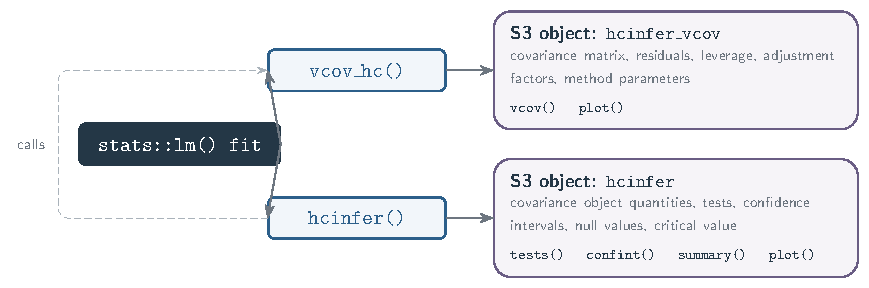
\includegraphics[width=1\linewidth,alt={Workflow diagram. A fitted lm() object feeds vcov_hc(), hcinfer(), boot_pairs(), and gls_mult(); hcinfer() internally calls vcov_hc(). vcov_hc() returns an hcinfer_vcov object supporting vcov() and plot(); hcinfer() returns an hcinfer object supporting tests(), confint(), summary(), and plot(); boot_pairs() returns an hcinfer_boot object supporting coef(), vcov(), confint(), and plot(); gls_mult() returns a gls_mult object supporting coef(), vcov(), tests(), confint(), summary(), plot(), logLik(), AIC(), BIC(), fitted(), and residuals().}]{figures/workflow} 

}

\caption{Main hcinfer workflow from a fitted lm() object to robust covariance estimation, coefficient inference, an empirical bootstrap reference, and a model-based variance alternative. The covariance object provides the robust covariance matrix, leverage values, adjustment factors, and method parameters; the inference object augments these with Wald tests and confidence intervals; the bootstrap object provides resampling standard errors and intervals; and the FGLS object provides model-based mean and dispersion estimates.}\label{fig:workflow}
\end{figure}

The same interface extends to two further entry points. The function \texttt{boot\_pairs(object,\ B,\ level,\ ci\_type,\ cores,\ seed)} produces pairs bootstrap standard errors and confidence intervals for the ordinary least squares coefficients, with reproducible resampling through \texttt{seed} and optional parallel execution through \texttt{cores}. The function \texttt{gls\_mult(object,\ variance,\ estimator,\ method,\ alpha,\ null)} fits feasible generalized least squares under a multiplicative variance model: \texttt{variance} supplies the dispersion regressors as a one-sided formula, \texttt{estimator} chooses Harvey's two-step procedure or Gaussian maximum likelihood, and \texttt{method} selects the optimizer for the likelihood fit. Both functions return S3 objects that reuse the same generics as the covariance and inference objects.

The available estimators are selected through \texttt{type}, and Table \ref{tab:methods} lists the implemented methods together with their tuning constants. These constants are supplied through \texttt{...} and default to the values proposed in the original methodology. This design allows the user to retune an estimator without changing the rest of the interface; for example, by setting \(k = 0.5\) for HC5 or \(c_1 = 5\) and \(c_2 = 0.5\) for \(\text{HC}_\beta\).

\begin{table}

\caption{\label{tab:methods}Heteroskedasticity-consistent covariance estimators implemented in the package. The values in the last column are the method-specific defaults exposed through the dots argument of the covariance and inference functions.}
\centering
\begin{tabular}[t]{ll>{\raggedright\arraybackslash}p{5.9cm}>{\raggedright\arraybackslash}p{3.7cm}}
\toprule
Type & Label & Description & Default arguments\\
\midrule
hc0 & HC0 & White heteroskedasticity-consistent estimator. & none\\
hc1 & HC1 & HC0 with degrees-of-freedom scaling. & none\\
hc2 & HC2 & Leverage-adjusted estimator with exponent 1. & none\\
hc3 & HC3 & Leverage-adjusted estimator with exponent 2. & none\\
hc4 & HC4 & Adaptive leverage correction by Cribari-Neto. & none\\
\addlinespace
hc4m & HC4m & Modified HC4 correction by Cribari-Neto and da Silva. & none\\
hc5 & HC5 & High-leverage correction by Cribari-Neto, Souza, and Vasconcellos. & k = 0.7\\
hc5m & HC5m & Modified HC5 correction by Li, Zhang, Zhang, and Wang. & k = 0.7, k1 = 1, k2 = 0, k3 = 1, gamma1 = 1, gamma2 = 1.5\\
hcbeta & HCbeta & Beta-distribution leverage correction. & c1 = 7, c2 = 0.75, lower = 0.01, upper = 0.99\\
\bottomrule
\end{tabular}
\end{table}

The tuning constants also make explicit the relationships among estimators. HC5m reduces to HC4m when \((k_1, k_2, k_3) = (1,1,0)\) and to HC5 when \((k_1, k_2, k_3) = (0,0,1)\). When the fitted shape parameters equal one, the beta CDF coincides with the uniform CDF; independently of those parameters, \(\text{HC}_\beta\) reduces exactly to HC1 when \(c_1=0\), because the adjustment exponent then vanishes. Methods without tuning constants do not accept additional arguments. For HC5, HC5m, and \(\text{HC}_\beta\), supplied argument names are validated against the documented set, so misspelled constants are rejected with an informative error rather than being ignored silently.

Table \ref{tab:api} lists the main user-facing functions. The package reuses the standard generics \texttt{coef()}, \texttt{vcov()}, \texttt{confint()}, \texttt{summary()}, \texttt{print()}, and \texttt{plot()}, allowing its objects to behave like familiar model outputs. The \texttt{plot()} method produces a coefficient forest plot for inference objects and an adjustment-factor diagnostic for covariance objects. Its \texttt{label\_top} argument controls how many high-leverage observations are annotated. The extractor functions \texttt{tests()} and \texttt{hc\_methods()} provide functionality beyond the base R generics, and both \texttt{tests()} and \texttt{confint()} accept a \texttt{parm} argument to restrict the output to selected coefficients. The \texttt{gls\_mult()} objects additionally support \texttt{logLik()}, \texttt{AIC()}, \texttt{BIC()}, \texttt{fitted()}, and \texttt{residuals()}, and the \texttt{boot\_pairs()} objects support \texttt{coef()}, \texttt{vcov()}, \texttt{confint()}, and \texttt{plot()}, so both behave like ordinary fitted-model outputs.

\begin{table}

\caption{\label{tab:api}Main user-facing functions in hcinfer.}
\centering
\begin{tabular}[t]{l>{\raggedright\arraybackslash}p{9.8cm}}
\toprule
Function & Role\\
\midrule
hcinfer() & Fits the full robust inference workflow for an lm() object.\\
vcov\_hc() & Returns the selected HC covariance matrix and diagnostics.\\
boot\_pairs() & Computes pairs (case) bootstrap standard errors and confidence intervals for OLS coefficients.\\
gls\_mult() & Fits feasible GLS under multiplicative heteroskedasticity by two-step or maximum likelihood.\\
tests() & Extracts coefficient-level normal Wald tests as a tibble.\\
\addlinespace
confint() & Extracts robust Wald confidence intervals.\\
summary() & Prints model metadata, method parameters, leverage diagnostics, robust weights, tests, and intervals.\\
plot() & Displays confidence intervals for inference objects or adjustment factors against leverage for covariance objects.\\
hc\_methods() & Lists implemented estimators and default method-specific arguments.\\
coef() and vcov() & Extract stored OLS coefficients and robust covariance matrices.\\
\bottomrule
\end{tabular}
\end{table}

\section{Implementation details}\label{implementation-details}

The implementation follows the sandwich representation in Equation \eqref{eq:sandwich}, but avoids two matrix constructions that would be unnecessarily expensive in routine use. The model matrix, residuals, coefficients, terms, model call, and formula are extracted once from the \texttt{lm()} object. Leverage values are obtained through \texttt{stats::hatvalues()}, which uses the QR decomposition stored in the fitted model, so the full hat matrix is never formed. This matters because the package only requires the diagonal entries \(h_t\), not the full \(n \times n\) matrix \(H\).

The covariance calculation also avoids forming \(\widehat{\Omega}\) as a dense diagonal matrix, and it applies the outer factors of the sandwich in Equation \eqref{eq:sandwich} without ever storing an inverse. Let \(A = X'X\), let \(\omega_t = \hat{e}_t^2 g_t\) collect the squared residuals and adjustment factors into the vector \(\boldsymbol{\omega} = (\omega_1, \ldots, \omega_n)'\), and let \(M = X'\operatorname{diag}(\boldsymbol{\omega})X\) denote the middle factor, so that the estimator becomes \(\widehat{\Psi}_{HC} = A^{-1} M A^{-1}\). Two evaluation paths return this matrix. A reference path first defines \texttt{A\_inv\ \textless{}-\ solve(crossprod(x))} and then evaluates the literal chain \texttt{A\_inv\ \%*\%\ t(x)\ \%*\%\ (x\ *\ omega)\ \%*\%\ A\_inv}; because the matrix product \texttt{\%*\%} has equal precedence and associates from left to right in R \citep{RCoreTeam2026}, the first product formed is \(A^{-1}X'\), a \(p \times n\) intermediate. The package path instead keeps \(\boldsymbol{\omega}\) as a vector, forms \(M\) directly with \texttt{crossprod(x,\ x\ *\ omega)}, and applies both outer factors through triangular solves. The two paths return the same covariance estimator in exact arithmetic, and the transcription below records the package sequence.

\begin{verbatim}
chol_solve <- function(chol_factor, b) {
  backsolve(
    chol_factor,
    forwardsolve(t(chol_factor), b)
  )
}
omega <- residuals^2 * weights
middle <- crossprod(x, x * omega)
xtx <- crossprod(x)
chol_factor <- chol(xtx) # tryCatch() guard omitted
left <- chol_solve(chol_factor, middle)
psi <- t(chol_solve(chol_factor, t(left)))
psi <- (psi + t(psi)) / 2
\end{verbatim}

These expressions make the working storage explicit without hiding a real allocation. R vector recycling evaluates \texttt{x\ *\ omega} as an \(n \times p\) row-scaled temporary, after which \texttt{crossprod(x,\ x\ *\ omega)} returns the required \(p \times p\) middle matrix directly, and \texttt{crossprod(x)} forms \(A\) without an explicit transpose at the R-expression level. Relative to the left-associated chain, the package path avoids the \(p \times n\) intermediate \(A^{-1}X'\), the explicit \texttt{t(x)} object, and the explicitly available inverse; both routes already avoid the conceptual dense \(n \times n\) matrix \(\widehat{\Omega}\) by scaling rows, whereas a literal transcription with \texttt{diag(omega)} would not. Beyond the model matrix and the vectors, the package expressions request one \(n \times p\) row-scaled design and \(p \times p\) intermediates, and the Cholesky factor replaces the inverse with another \(p \times p\) object. Omitting the inverse alone is therefore not an asymptotic reduction in memory; these are statements about the shapes of the objects created rather than measurements of peak memory.

The two paths also differ in the number of scalar multiplications used to assemble the sandwich. We adopt a dense-arithmetic convention in which, once \(\boldsymbol{\omega}\) is available, the count retains only the dominant assembly terms that depend on \(n\), treats the symmetric one-argument cross-product \(X'X\) as a single triangle, and includes the common \(np\) row scaling, while excluding transpositions, additions, lower-order vector work, backend effects, and the route-specific \(O(p^3)\) work. Under this convention the leading counts are
\begin{equation}
\begin{aligned}
C_{\mathrm{left}}^{(n)} &= np(p+1)/2 + np + 2np^2, \\
C_{\mathrm{hcinfer}}^{(n)} &= np(p+1)/2 + np + np^2,
\end{aligned}
\label{eq:assembly-counts}
\end{equation}
with leading totals \(\tfrac{5}{2}np^2\) and \(\tfrac{3}{2}np^2\). The counts in Equation \eqref{eq:assembly-counts} differ by one classical \(np^2\) multiplication stage, so forming \(M\) directly removes that stage relative to the left-associated chain. Both paths nonetheless remain \(O(np^2 + p^3)\), and the package's \(p^3\) contribution consists of one factorization together with four triangular-solve calls carrying \(p\) right-hand-side columns. The ratio \(5/3\) compares the leading \(n\)-dependent coefficients and is not a universal wall-clock speed ratio, and an explicit-inverse expression that forms \(M\) before applying the inverse shares the package route's leading \(n\)-dependent count, so the comparison does not extend to every inverse-based evaluation order.

The factorized route applies \(A^{-1}\) twice through the same Cholesky factor. The call \texttt{chol(xtx)} produces \(A = R'R\) with \(R\) upper triangular, and each application of \texttt{chol\_solve()} performs one forward and one backward triangular-solve call on a \(p \times p\) matrix right-hand side. The first helper call solves \(AL = M\) and yields \(L = A^{-1}M\), the second solves \(AZ = L'\) and yields \(Z = A^{-1}L'\), and transposition then gives \(Z' = A^{-1}MA^{-1}\) because \(A\) and \(M\) are symmetric. Each covariance call therefore performs four triangular-solve calls, two forward and two backward, reusing one factorization for the two applications of \(A^{-1}\) and storing no inverse. Solving with the factor rather than constructing \(A^{-1}\) for later multiplication follows standard numerical-linear-algebra practice \citep{Higham2002}, although it establishes no measured accuracy gain, no stability theorem for the full covariance calculation, and no immunity to collinearity. Because \(\kappa_2(X'X) = \kappa_2(X)^2\) for full-column-rank \(X\), the conditioning of the normal-equations matrix remains part of both paths.

The factorization is wrapped in a \texttt{tryCatch()} call whose role is deliberately narrow. It reports when the computed cross-product is not numerically positive definite, so it is a factorization-failure guard rather than a condition-number diagnostic, and a successful factorization does not establish that \(X\) or \(X'X\) is well conditioned. Averaging the result with its transpose in the final line enforces exact symmetry of the returned matrix; this step is neither a conditioning check nor a positive-semidefiniteness check, and it does not establish improved numerical accuracy of the symmetric part. These safeguards are separate from the broader input validation described later in this section, which screens the fitted model before the covariance routine runs.

The package tests bound these claims narrowly rather than certifying them in general. They include one regression check that compares the HC3 covariance against the direct expression \(A^{-1} X'\operatorname{diag}(\boldsymbol{\omega})X A^{-1}\) at tolerance \(10^{-10}\), together with a separate check that the returned \(\text{HC}_\beta\) matrix equals its own transpose. The direct expression is an alternate double-precision route rather than a high-precision oracle, so the agreement it confirms is consistency between two finite-precision computations of the same estimator. The comparison in this section is analytical rather than a wall-clock benchmark, an allocation profile, or an empirical accuracy experiment; repeated covariance calls can make the avoided product and the avoided allocation relevant, yet the manuscript claims neither a general speedup nor that this helper determined the runtime or numerical reliability of any other analysis. Figure \ref{fig:sandwich-efficiency} summarizes this data flow, tracing the inputs through the two construction branches to the triangular solves and the symmetrized output.

\begin{figure}

{\centering 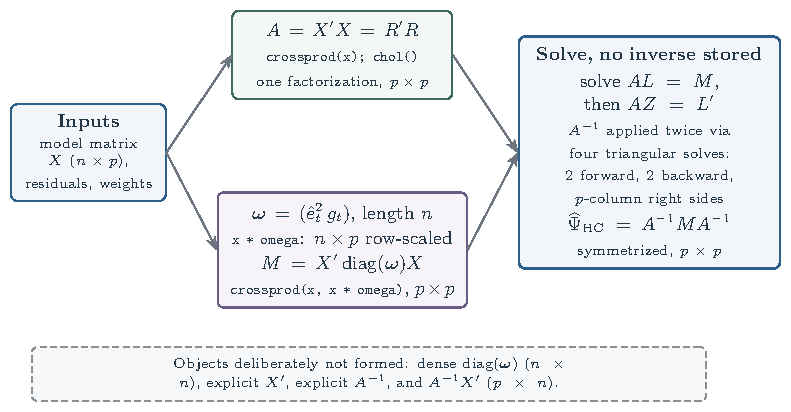
\includegraphics[alt={Left-to-right data-flow diagram of the hcinfer covariance calculation. On the left, the inputs are the model matrix X of size n by p, the residual vector, and the weight vector. The flow splits into two branches. The upper branch forms the cross-product A equal to X-transpose times X of size p by p and its Cholesky factor R. The lower branch keeps the weights as the length-n vector omega, materializes the row-scaled design x times omega as an n by p temporary, and returns the middle matrix M equal to X-transpose times diag(omega) times X directly as p by p. The two branches meet only at a solve node that performs four triangular-solve calls on matrix right-hand sides, two forward and two backward, applying the inverse of A twice without storing it, and then symmetrizes the p by p covariance output. Below the flow, a separate dashed box with no arrows into or out of it lists the objects deliberately not formed: the dense n by n diagonal matrix, the explicit transpose of X, the explicit inverse of A, and the p by n product formed by the inverse of A times X-transpose.}]{figures/sandwich-efficiency} 

}

\caption{Factorized covariance data flow in hcinfer. The diagonal is retained as the vector $\boldsymbol{\omega}$, and R materializes the row-scaled design $\operatorname{diag}(\boldsymbol{\omega})X$ as an $n \times p$ temporary before the cross-product returns the middle matrix $M = X'\operatorname{diag}(\boldsymbol{\omega})X$ as $p \times p$. The upper branch forms $A = X'X$ and a single Cholesky factor, and the two branches meet in four triangular-solve calls, two forward and two backward on matrix right-hand sides, followed by symmetrization of the output. The dashed annotation lists the objects the routine deliberately does not form rather than another step in the flow.}\label{fig:sandwich-efficiency}
\end{figure}

HC weights are computed by a single vectorized dispatcher. The dispatcher constructs \(h_t/\bar{h}\), \(1-h_t\), and \(h_{\max}\) once and changes only the formula for \(g_t\). This keeps the estimators comparable in code as well as in the underlying mathematics: HC0 through HC5m and \(\text{HC}_\beta\) all enter the same sandwich calculation after their adjustment factors have been computed.

The feasible generalized least squares routine \texttt{gls\_mult()} reuses the same computational discipline as the covariance calculation. It never forms the \(n\times n\) weight matrix \(\widehat W\); instead it row-scales the design by the weight vector, centers the fitted log-variances to improve conditioning, and solves the weighted normal equations through a Cholesky factorization rather than an explicit inverse. For the maximum likelihood fit it profiles \(\boldsymbol{\beta}\) out by weighted least squares and optimizes only the \(q\) dispersion parameters with the analytic profile gradient, and it accepts a solution as a local optimum only when the optimizer converges and the scale-invariant profile-score norm falls below a fixed tolerance, which rejects a false convergence report at a nonstationary point.

The pairs bootstrap \texttt{boot\_pairs()} draws all resampling indices once in the main process under the supplied \texttt{seed} and refits each replicate with \texttt{stats::.lm.fit()}, so the result is deterministic and independent of the number of cores. When more than one core is requested, the deterministic replicate fits are distributed with \texttt{purrr::in\_parallel()} and the \CRANpkg{mirai} backend without changing the numeric result. Rank-deficient resamples are detected by their reduced rank and dropped, and the call stops if fewer than two valid replicates remain.

Validation is performed early and specifically. The package rejects rank-deficient models, models with \(p \ge n\), non-finite coefficients or residuals, leverage values outside the admissible interval, and cases where \(1-h_t\) is numerically nonpositive. For HC5, HC5m, and \(\text{HC}_\beta\), method constants supplied through \texttt{...} are checked against their allowed names and scalar constraints. For \(\text{HC}_\beta\), the truncation limits must lie in \((0,1)\), the lower limit must be smaller than the upper limit, the estimated beta parameters must be positive and finite, and the final weights must be positive and finite.

The \(\text{HC}_\beta\) implementation estimates the beta parameters by the method of moments from the truncated leverage complements \(w_t\), and then applies the shrinkage defined in Equation \eqref{eq:shrinkage}. The regularized incomplete beta function is not reimplemented in the package; instead, the numerically stable base R routine \texttt{stats::pbeta()} is used directly. This choice keeps the implementation short and delegates a delicate numerical routine to a well-tested standard library function.

The package returns S3 objects rather than plain matrices whenever diagnostics are required. Objects of class \texttt{hcinfer\_vcov} store covariance-level quantities, including the covariance matrix, residuals, leverage values, adjustment factors, method parameters, and model metadata. Objects of class \texttt{hcinfer} add the coefficient-level inferential table, null values, confidence level, and critical value, so that print, summary, plot, and extractor methods base their output on these shared structures. This common storage model keeps the reported inference and diagnostics tied to the same covariance calculation.

The package dependencies are intentionally small and targeted. The \CRANpkg{cli} package formats console output \citep{Cli2026}, \CRANpkg{tibble} stores tabular results \citep{Tibble2026}, \CRANpkg{ggplot2} builds graphics \citep{Wickham2016Ggplot2}, and \CRANpkg{purrr} and \CRANpkg{rlang} support functional programming and argument validation \citep{Purrr2026, Rlang2026}. Figure \ref{fig:architecture} maps the implementation files and package assets in the GitHub repository.

\begin{figure}

{\centering 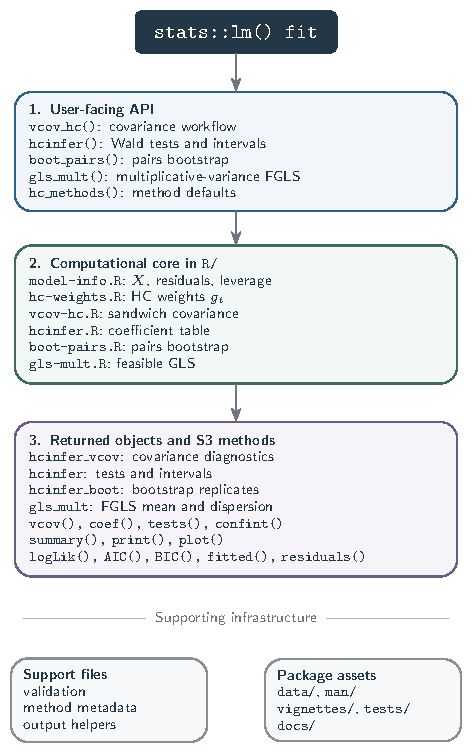
\includegraphics[alt={Architecture diagram. A fitted lm() object feeds a user-facing API layer with vcov_hc(), hcinfer(), boot_pairs(), gls_mult(), and hc_methods(). This drives a computational core of model-info.R, hc-weights.R, vcov-hc.R, hcinfer.R, boot-pairs.R, and gls-mult.R, which produces returned objects and S3 methods: hcinfer_vcov, hcinfer, hcinfer_boot, and gls_mult, with vcov(), coef(), tests(), confint(), summary(), print(), plot(), logLik(), AIC(), BIC(), fitted(), and residuals(). Supporting infrastructure below covers support files and package assets such as data/, man/, vignettes/, tests/, and docs/.}]{figures/architecture} 

}

\caption{Repository-level architecture of hcinfer. The diagram separates the public API, the computational core, the S3 output layer, and the surrounding support files and package assets.}\label{fig:architecture}
\end{figure}

Figure \ref{fig:logo} shows the \CRANpkg{hcinfer} package logo. At submission, version 0.3.0 is on CRAN, the GitHub repository hosts the development source, and documentation is available on the package website. The package can be installed from CRAN, from r-universe, or from the GitHub development repository; the GitHub route uses \CRANpkg{remotes} \citep{Remotes2024}. Together, these channels provide distinct access points for the stable release, the development source, and the package documentation.

\begin{figure}

{\centering 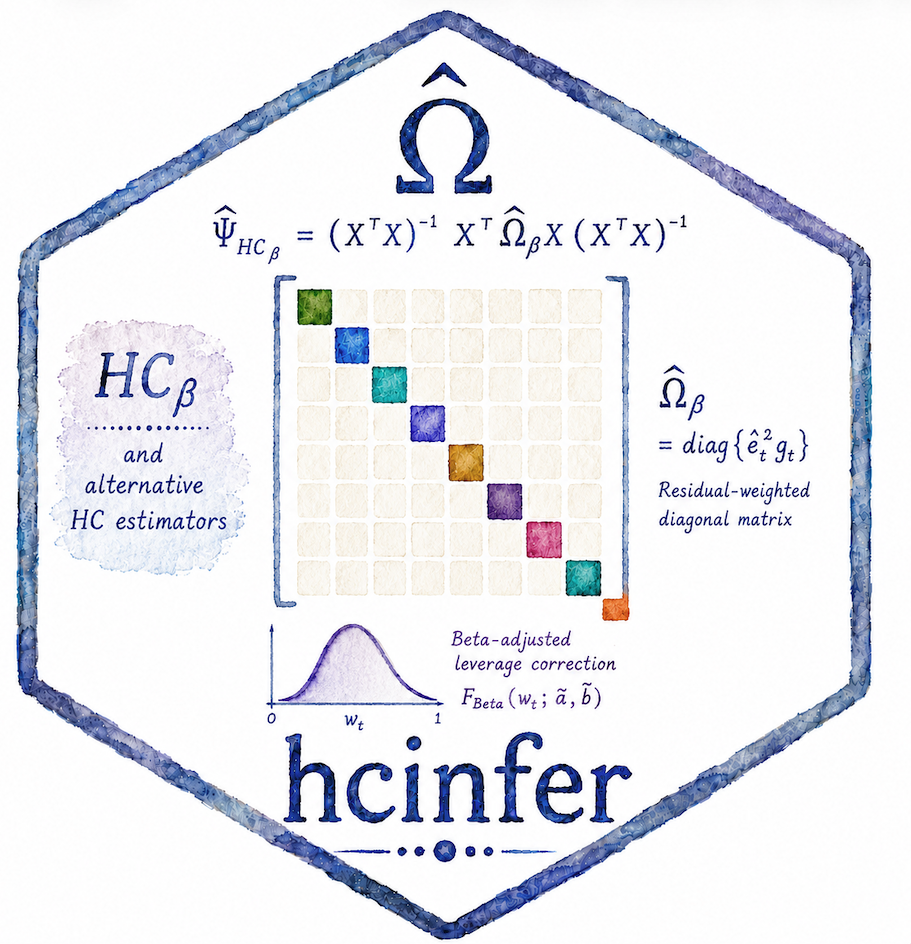
\includegraphics[width=0.32\linewidth,alt={The hcinfer package logo.}]{figures/logo} 

}

\caption{The hcinfer package logo. The package implements heteroskedasticity-consistent inference for linear models; suggestions and improvements are welcome through GitHub issues and pull requests.}\label{fig:logo}
\end{figure}

The package can be installed in three ways depending on whether a stable release or a development snapshot is preferred. CRAN provides the published release, while r-universe and GitHub provide current development builds. The non-evaluated commands below document each route without changing the reader's R library during article rendering.

\begin{verbatim}
install.packages("hcinfer")
install.packages("hcinfer", repos = c(
  "https://prdm0.r-universe.dev",
  "https://cloud.r-project.org"
))
remotes::install_github("prdm0/hcinfer", force = TRUE)
\end{verbatim}

\section{Worked example}\label{worked-example}

To illustrate the use of the package in a practical setting, we consider data on public education expenditures across the U.S. states. The dataset, included in the package, contains three variables. The response variable \texttt{expenditure} is the annual K-12 per-pupil spending, measured in U.S. dollars. These expenditures include instructional costs, teacher salaries and benefits, administrative expenses, support staff, transportation, and facilities, with 2025 as the reference year. The variable \texttt{income} is the 2024 nominal per capita income for each state, as reported by the \emph{Bureau of Economic Analysis}. Finally, \texttt{south} is a regional indicator variable. The values of the two continuous variables were obtained from the \emph{World Population Review} and refer to 2024; the data refer to the 50 U.S. states plus the District of Columbia.
The \texttt{south} indicator takes the value 1 for the Southern states (Alabama, Arkansas, Delaware, Florida, Georgia, Kentucky, Louisiana, Maryland, Mississippi, North Carolina, Oklahoma, South Carolina, Tennessee, Texas, Virginia, and West Virginia) as well as the District of Columbia (a federal district classified by the \emph{Census Bureau} as part of the \emph{South Atlantic} subregion), and 0 otherwise.

We consider the intercept-free linear regression model given by
\begin{equation}
y_t = \beta_2 x_{t2} + \beta_3 x_{t2} x_{t3} + e_t, \quad t = 1, \ldots, 51,
\label{eq:educ}
\end{equation}
where \(y_t\) denotes the annual per-pupil spending in jurisdiction \(t\), and \(x_{t2}\) is per capita income scaled by \(10^{-4}\) for numerical convenience (that is, measured in units of ten thousand dollars). The variable \(x_{t3}\) is the regional indicator, taking the value 1 for Southern states and 0 otherwise, while \(x_{t2}x_{t3}\) is the interaction term between scaled income and Southern-region membership. The intercept-free specification in Equation \eqref{eq:educ} is motivated by the natural proportionality between educational expenditures and per capita income. It is reasonable to assume that, in the complete absence of income, the expected per-pupil expenditure would also be zero.

\begin{verbatim}
library(hcinfer)

data("PublicSchools2", package = "hcinfer")
df <- PublicSchools2
df$scaled_income <- df$income / 10000

fit    <- lm(expenditure ~ scaled_income + scaled_income:south - 1, data = df)
result <- hcinfer(fit)
\end{verbatim}

The ordinary least squares estimates are \(\hat{\beta}_2 = 4100.65\) and \(\hat{\beta}_3 = -322.66\). The estimate of \(\hat{\beta}_2\) indicates that an increase of \$10,000 in per capita income is associated with an increase of \$4100.65 in average annual per-pupil spending for jurisdictions outside the South. The negative sign of \(\hat{\beta}_3\) suggests that Southern states spend less per pupil than non-Southern states with the same level of per capita income. The primary objective is to test the null hypothesis \(\mathcal{H}_0 \colon \beta_3 = 0\) against the alternative hypothesis \(\mathcal{H}_1 \colon \beta_3 \neq 0\). Under the null hypothesis, the effect of income on educational spending is the same across all regions. Under the alternative, the South exhibits a different regional pattern.

Figure \ref{fig:scatter} displays the scatter plot together with the fitted regression lines, allowing a visual comparison of these two scenarios. The plot reveals a clear positive linear association between per capita income and per-pupil spending. Observations from the South (\(x_{t3}=1\)) and from the remaining regions (\(x_{t3}=0\)) follow the same overall trend. The fitted regression lines obtained by setting the indicator variable equal to one and zero closely track the full set of observations in both regions, and the slopes of the two fitted lines are similar throughout the range of the data. This visual pattern provides preliminary evidence that there is no meaningful regional difference.

\begin{figure}

{\centering 
\includegraphics[alt={Scatter plot of expenditure against scaled per capita income. Points are colored by region. Two fitted regression lines, constrained to pass through the origin, are overlaid: one for Southern states and one for the remaining states. The two lines have similar positive slopes over the range of the data.}]{hcinfer_files/figure-latex/scatter-1} 

}

\caption{Scatter plot and fitted regression lines (constrained to pass through the origin) relating annual K-12 per-pupil spending to per capita income for Southern states and the remaining U.S. states.}\label{fig:scatter}
\end{figure}

The \texttt{hcinfer()} function returns all the quantities required for statistical inference. The \texttt{confint()} and \texttt{tests()} methods extract the robust confidence intervals and Wald test results, respectively. Both methods return tibbles that can be filtered or combined with results from other covariance estimators.

\begin{verbatim}
confint(result)
\end{verbatim}

\begin{verbatim}
#> # A tibble: 2 x 4
#>   term                conf_low conf_high level
#>   <chr>                  <dbl>     <dbl> <dbl>
#> 1 scaled_income          3785.     4417.  0.95
#> 2 scaled_income:south    -822.      176.  0.95
\end{verbatim}

\begin{verbatim}
tests(result)[c("term", "std_error", "z_value", "p_value")]
\end{verbatim}

\begin{verbatim}
#> # A tibble: 2 x 4
#>   term                std_error z_value   p_value
#>   <chr>                   <dbl>   <dbl>     <dbl>
#> 1 scaled_income            161.   25.4  1.23e-142
#> 2 scaled_income:south      255.   -1.27 2.05e-  1
\end{verbatim}

The \(\text{HC}_\beta\) standard error of \(\hat{\beta}_3\) is \(254.58\), and the corresponding Wald statistic for testing \(\beta_3 = 0\) is \(z = -1.27\), with a \(p\)-value of \(0.205\). Accordingly, the test based on the \(\text{HC}_\beta\) estimator does not reject the null hypothesis at the 10\% significance level. By contrast, the corresponding test for the coefficient \(\beta_2\) provides strong evidence against the null hypothesis, with \(z = 25.43\) and \(p\)-value \(< 0.0001\), confirming a positive association between per capita income and annual per-pupil spending regardless of region. The 95\% \(\text{HC}_\beta\) confidence interval for \(\beta_3\) is \([-821.62, 176.31]\), which is consistent with the absence of evidence against the null hypothesis.

Model selection criteria reinforce these findings. The model including the interaction term yields an adjusted \(R^2\) of \(0.9650\), an \(\mathrm{AIC}\) (Akaike information criterion) of \(978.43\), and a \(\mathrm{BIC}\) (Bayesian information criterion) of \(984.22\). The simpler model without the interaction term (\(y_t = \beta_2 x_{t2} + e_t\)) has an adjusted \(R^2\) of \(0.9643\), the same \(\mathrm{AIC}\) value of \(978.43\), and a smaller \(\mathrm{BIC}\) of \(982.29\). Thus, including the interaction term produces virtually no improvement in the adjusted \(R^2\) while slightly increasing the BIC. These model selection criteria are therefore consistent with the conclusion drawn from the Wald test. From the standpoint of model selection and the principle of parsimony, the simpler model without the regional interaction is preferable.

The \texttt{summary()} method consolidates the results into a single output. It reports model metadata, including the selected covariance estimator, observation leverages, adjustment factors, and the tables of hypothesis tests and confidence intervals. When the \(\text{HC}_\beta\) estimator is used, the output also reports the estimated beta-distribution parameters (here, \(\tilde{a} = 27.57\) and \(\tilde{b} = 1.60\)). The \texttt{plot()} method produces a forest plot displaying the confidence intervals for the regression coefficients. Figure \ref{fig:intervals} shows this plot for the education-expenditure regression.

\begin{figure}

{\centering 
\includegraphics[alt={Forest plot of HCbeta confidence intervals for the two regression coefficients. Each row shows a horizontal interval with a point estimate and a vertical dashed line marking the null value used for the Wald tests.}]{hcinfer_files/figure-latex/intervals-1} 

}

\caption{HCbeta confidence intervals for the coefficients of the education-expenditure regression (intercept-free model). The vertical dashed line indicates the null value used in the coefficient-level hypothesis tests.}\label{fig:intervals}
\end{figure}

With \(p = 2\) regression coefficients and \(n = 51\) observations, the average leverage is \(\bar{h} = p/n \approx 0.039\). The most commonly used thresholds for identifying leverage points are \(2p/n \approx 0.078\) and \(3p/n \approx 0.118\). The leverage values of three jurisdictions exceed the lower threshold of \(2p/n\): the District of Columbia (\(h_9 = 0.188\)), Maryland (\(h_{21} = 0.088\)), and Virginia (\(h_{47} = 0.081\)). Only the District of Columbia exceeds the more stringent threshold of \(3p/n\), identifying it as a high-leverage observation. Maryland and Virginia fall into an intermediate range and may be regarded as moderately high-leverage observations. Notably, both belong to the Southern region and therefore contribute to the interaction term in the fitted model.

These leverage values are readily explained by the underlying data. The District of Columbia is located between Maryland and Virginia and has a 2024 per capita income of \$77,348, the highest value in the sample. This combination of exceptionally high income and membership in the Southern group places it far from the bulk of the observations in the predictor space, causing its leverage to exceed the \(3p/n\) threshold. Consequently, it is the most atypical design point in the dataset from the perspective of leverage.

The vector of leverage values can be extracted from the object returned by \texttt{vcov\_hc()} and is also available in the object returned by \texttt{hcinfer()}. Comparing these values with conventional thresholds identifies observations that warrant closer inspection. The evaluated code below separates moderate and high-leverage cases for the fitted model.

\begin{verbatim}
cov_hcbeta <- vcov_hc(fit, type = "hcbeta")
h <- cov_hcbeta$leverage
p <- 2
n <- length(h)

# Mild leverage (> 2p/n and <= 3p/n)
unname(which(h > 2 * p / n & h <= 3 * p / n))
\end{verbatim}

\begin{verbatim}
#> [1] 21 47
\end{verbatim}

\begin{verbatim}
# High leverage (> 3p/n)
unname(which(h > 3 * p / n))
\end{verbatim}

\begin{verbatim}
#> [1] 9
\end{verbatim}

The visual diagnostic for the adjustment factors can be obtained via the \texttt{plot()} method applied to a covariance object. This call is evaluated to verify the method while its single-method plot is hidden, because Figure \ref{fig:weights} provides the more informative four-method comparison. The code remains visible so readers can reproduce the individual diagnostic interactively.

\begin{verbatim}
plot(cov_hcbeta)
\end{verbatim}

Figure \ref{fig:weights} displays the adjustment factors \(g_t\) used by the HC3, HC4, HC4m, and \(\text{HC}_\beta\) estimators as functions of the leverage values (\(h_t\)). The panels use different vertical scales, each determined by the range of the corresponding adjustment factors. For the District of Columbia, HC4 multiplies the squared residual by a factor of \(2.30\), HC4m uses a factor of \(1.68\), and HC3 applies a factor of \(1.52\). By contrast, the \(\text{HC}_\beta\) estimator uses an adjustment factor of \(5.52\). This difference arises because \(\text{HC}_\beta\) does not base its correction solely on the leverage of an individual observation. Instead, it incorporates the entire empirical distribution of the leverage values through a fitted beta distribution, producing an adjustment that can be larger than fixed-power corrections for the most influential points without growing unboundedly with extreme leverage.

\begin{figure}

{\centering 
\includegraphics[alt={Four-panel scatter plot of adjustment factors against leverage for HC3, HC4, HC4m, and HCbeta. Each panel uses a free vertical scale. A dashed vertical line marks the 3p/n high-leverage threshold. Points beyond the threshold are highlighted in red.}]{hcinfer_files/figure-latex/weights-1} 

}

\caption{Adjustment factors $g_t$ versus leverage values $h_t$ for the education-expenditure regression (intercept-free model with an interaction term). Red points correspond to observations whose leverage exceeds the conventional high-leverage threshold of $3p/n$.}\label{fig:weights}
\end{figure}

Table \ref{tab:comparison} summarizes the robust inference for the coefficient \(\beta_3\) obtained from the nine covariance estimators implemented in the package. For each estimator, the table reports the robust standard error, the \(p\)-value for the test of \(\mathcal{H}_0 \colon \beta_3 = 0\), the largest adjustment factor \(g_t\), and the corresponding 95\% confidence interval. The robust standard errors range from \(194.58\) (HC0) to \(254.58\) (\(\text{HC}_\beta\)). This variation reflects the different ways in which the estimators account for the high-leverage District of Columbia observation. At the 5\% significance level, all nine tests lead to the same conclusion that there is no evidence that the effect of per capita income on educational spending differs between the two regions. At the 10\% level, however, the HC0-based test rejects the null hypothesis (\(p\)-value \(=0.097\)), illustrating how inference can depend on the covariance estimator when a high-leverage observation is present.

\begin{table}

\caption{\label{tab:comparison}Robust inference for the income-South interaction coefficient in the public school expenditure regression, intercept-free model. The OLS estimate is -322.66, and income is scaled to units of ten thousand U.S. dollars.}
\centering
\begin{tabular}[t]{lllll}
\toprule
Estimator & Standard error & p-value & max g\_t & 95\% CI\\
\midrule
HC0 & 194.5776 & 0.0973 & 1.0000 & {}[-704.0, 58.7]\\
HC1 & 198.5089 & 0.1041 & 1.0408 & {}[-711.7, 66.4]\\
HC2 & 200.4590 & 0.1075 & 1.2318 & {}[-715.5, 70.2]\\
HC3 & 206.8074 & 0.1187 & 1.5173 & {}[-728.0, 82.7]\\
HC4 & 210.3112 & 0.1250 & 2.3023 & {}[-734.9, 89.5]\\
\addlinespace
HC4m & 208.5696 & 0.1219 & 1.6840 & {}[-731.4, 86.1]\\
HC5 & 210.3112 & 0.1250 & 2.3023 & {}[-734.9, 89.5]\\
HC5m & 218.1235 & 0.1391 & 2.8360 & {}[-750.2, 104.9]\\
HCbeta & 254.5770 & 0.2050 & 5.5185 & {}[-821.6, 176.3]\\
\bottomrule
\end{tabular}
\end{table}

To assess the robustness of the inference for the coefficient \(\beta_3\), we examine the effect of removing the District of Columbia from the sample. Excluding this observation changes the ordinary least squares estimates to \(\hat{\beta}_2 = 4100.65\) and \(\hat{\beta}_3 = -394.79\). Figure \ref{fig:weights-nodc} displays the corresponding adjustment factors for this reduced sample. In this setting, no observation exceeds the conventional high-leverage threshold of \(3p/n\). The only jurisdictions with leverage values above the moderate threshold of \(2p/n\) are Maryland and Virginia. Both belong to the Southern region and therefore contribute to the interaction term, with Maryland becoming the highest-leverage observation (\(h_{21} = 0.109\)).

\begin{figure}

{\centering 
\includegraphics[alt={Four-panel scatter plot of adjustment factors against leverage for HC3, HC4, HC4m, and HCbeta fitted on the subsample without the District of Columbia. A dashed vertical line marks the 3p/n threshold; no points are highlighted as high leverage.}]{hcinfer_files/figure-latex/weights-nodc-1} 

}

\caption{Adjustment factors $g_t$ plotted against leverage values $h_t$ for the intercept-free model with an interaction term, fitted to the subsample excluding the District of Columbia. Because no observation exceeds the common high-leverage threshold of $3p/n$, the adjustment factors vary more smoothly across the sample, and the plot() method does not highlight any observations in red.}\label{fig:weights-nodc}
\end{figure}

Table \ref{tab:comparison-nodc} reports the robust standard errors of \(\hat{\beta}_3\), the \(p\)-values for testing \(\mathcal{H}_0\colon \beta_3 = 0\), the largest adjustment factors \(g_t\), and the corresponding 95\% confidence intervals based on the reduced dataset. After removing the District of Columbia, the tests based on the HC0, HC1, HC2, HC3, HC4, HC4m, HC5, and HC5m estimators all reject the null hypothesis at the 10\% significance level. In sharp contrast, the inference based on the \(\text{HC}_\beta\) estimator remains essentially unchanged, yielding a \(p\)-value of \(0.118\) and therefore continuing to reject neither the null hypothesis at the 10\% level nor at the more stringent 5\% level. Notably, this is the same inferential conclusion obtained from the full sample, which suggests that the \(\text{HC}_\beta\) correction is comparatively stable in the presence of the high-leverage observation rather than being driven by it.

\begin{table}

\caption{\label{tab:comparison-nodc}Robust inference for the interaction coefficient in the subsample excluding the District of Columbia, intercept-free model. The OLS estimate is -394.79 and the subsample has n = 50 observations.}
\centering
\begin{tabular}[t]{lllll}
\toprule
Estimator & Standard error & p-value & max g\_t & 95\% CI\\
\midrule
HC0 & 201.8961 & 0.0505 & 1.0000 & {}[-790.5, 0.9]\\
HC1 & 206.0593 & 0.0554 & 1.0417 & {}[-798.7, 9.1]\\
HC2 & 207.3460 & 0.0569 & 1.1220 & {}[-801.2, 11.6]\\
HC3 & 213.0049 & 0.0638 & 1.2589 & {}[-812.3, 22.7]\\
HC4 & 210.5388 & 0.0608 & 1.3675 & {}[-807.4, 17.9]\\
\addlinespace
HC4m & 214.3843 & 0.0655 & 1.3335 & {}[-815.0, 25.4]\\
HC5 & 210.5388 & 0.0608 & 1.3675 & {}[-807.4, 17.9]\\
HC5m & 216.0995 & 0.0677 & 1.5344 & {}[-818.3, 28.8]\\
HCbeta & 252.4793 & 0.1179 & 3.2007 & {}[-889.6, 100.1]\\
\bottomrule
\end{tabular}
\end{table}

An alternative way to assess the influence of the District of Columbia on the inference is to retain this observation in the dataset while changing only its regional classification. When the District of Columbia is no longer classified as part of the South, the ordinary least squares estimate becomes \(\hat{\beta}_3 = -393.89\). The corresponding \(\text{HC}_\beta\) standard error is \(241.23\), and the resulting Wald test yields a \(p\)-value of \(0.102\). Thus, the inferential conclusion remains unchanged.

As an additional sensitivity analysis, we consider the corresponding regression model with an intercept. The ordinary least squares estimates are \(\hat{\beta}_1 = -3813.72\), \(\hat{\beta}_2 = 4932.66\), and \(\hat{\beta}_3 = -299.07\). Under the \(\text{HC}_\beta\) covariance estimator, the corresponding standard errors are \(2015.94\), \(493.44\), and \(205.20\), yielding \(p\)-values of \(0.059\), \(1.58 \times 10^{-23}\), and \(0.145\), respectively. The intercept is therefore not statistically significant at the 5\% level, providing further support for the intercept-free specification adopted throughout the analysis.

Table \ref{tab:gt-comparison} compares the largest adjustment factors \(g_t\) under the intercept-free and intercept models. Including an intercept increases the leverage values, with the District of Columbia reaching \(h_9 = 0.555\), well above the common high-leverage threshold of \(3p/n = 0.176\). The classical HC estimators respond very differently to this increase. Under HC4, the largest adjustment factor rises from \(2.30\) to \(25.39\). For HC5, it increases from \(2.30\) to \(207.66\), and for HC5m from \(2.84\) to \(466.15\). By contrast, the corresponding maximum under \(\text{HC}_\beta\) changes only marginally, from \(5.52\) to \(5.29\). This comparison illustrates that, even in the presence of extremely high leverage, the \(\text{HC}_\beta\) estimator produces remarkably stable adjustment factors, in marked contrast to the classical HC estimators whose correction grows rapidly with leverage.

\begin{table}

\caption{\label{tab:gt-comparison}Maximum adjustment factor $g_t$ for the interaction coefficient under the intercept-free and intercept models. The intercept-free model is $y_t = \beta_2 x_{t2} + \beta_3 x_{t2} x_{t3} + e_t$ and the intercept model is $y_t = \beta_1 + \beta_2 x_{t2} + \beta_3 x_{t2} x_{t3} + e_t$. HCbeta maintains stable adjustment factors across the two specifications.}
\centering
\begin{tabular}[t]{lll}
\toprule
Estimator & max g\_t (no intercept) & max g\_t (with intercept)\\
\midrule
HC0 & 1.00 & 1.00\\
HC1 & 1.04 & 1.06\\
HC2 & 1.23 & 2.24\\
HC3 & 1.52 & 5.04\\
HC4 & 2.30 & 25.39\\
\addlinespace
HC4m & 1.68 & 7.55\\
HC5 & 2.30 & 207.66\\
HC5m & 2.84 & 466.15\\
HCbeta & 5.52 & 5.29\\
\bottomrule
\end{tabular}
\end{table}

\subsection{A bootstrap reference and a variance model}\label{a-bootstrap-reference-and-a-variance-model}

The primary \(\text{HC}_\beta\) analysis can be complemented by two tools that operate on the same fitted model \texttt{fit}. The pairs bootstrap in \texttt{boot\_pairs()} resamples whole jurisdictions and refits ordinary least squares, providing an assumption-free empirical reference for the analytic standard errors, while \texttt{gls\_mult()} fits a multiplicative-variance model that estimates the heteroskedasticity explicitly and reweights the observations. Because the mean model is intercept-free, the dispersion model is supplied as the one-sided formula \texttt{\textasciitilde{}\ scaled\_income}, which lets the error variance grow with per capita income and provides the intercept that the dispersion model requires.

\begin{verbatim}
boot <- boot_pairs(fit, B = 2000, seed = 2026)
gls_fit <- gls_mult(fit, variance = ~ scaled_income)
\end{verbatim}

All 2000 resamples produced a full-rank fit, so no replicate was discarded. The pairs bootstrap standard error of the interaction coefficient \(\beta_3\) is 201.91, and that of the income slope \(\beta_2\) is 147.94. For both coefficients the bootstrap standard error lies between the HC0 and HC3 values and below the more conservative \(\text{HC}_\beta\) standard error, as Table \ref{tab:fgls-se} shows. The resampling reference therefore corroborates the analytic heteroskedasticity-consistent standard errors for these coefficients without relying on any variance model.

The default maximum likelihood fit of \texttt{gls\_mult()} re-estimates the coefficients under the fitted variance model. The mean estimates are 4005.30 for the income slope and -261.26 for the interaction, close to the ordinary least squares estimates reported earlier, with model-based standard errors of 127.64 and 212.97. The interaction remains statistically indistinguishable from zero, so the substantive conclusion of the \(\text{HC}_\beta\) analysis is unchanged. The positive log-variance slope on scaled income (0.79) indicates that the conditional variance increases with per capita income, and because a maximum likelihood fit carries a genuine log-likelihood, its \texttt{AIC()} of 976.92 and \texttt{BIC()} of 984.65 allow direct comparison of competing variance specifications. Since its covariance is model based, \texttt{gls\_mult()} complements rather than replaces the heteroskedasticity-consistent estimators.

\begin{table}

\caption{\label{tab:fgls-se}Standard errors for the two coefficients of the intercept-free interaction model, where $\beta_2$ is the scaled-income slope and $\beta_3$ the interaction between scaled income and the Southern-region indicator. The OLS, HC, and pairs bootstrap rows all summarize the same ordinary least squares coefficient estimates, whereas FGLS (ML) re-estimates the coefficients under the multiplicative variance model, so its standard errors refer to different point estimates.}
\centering
\begin{tabular}[t]{lll}
\toprule
Method & SE(scaled\_income) & SE(scaled\_income:south)\\
\midrule
OLS & 128.51 & 230.44\\
HC0 & 145.88 & 194.58\\
HC3 & 150.69 & 206.81\\
HCbeta & 161.26 & 254.58\\
Pairs bootstrap & 147.94 & 201.91\\
\addlinespace
FGLS (ML) & 127.64 & 212.97\\
\bottomrule
\end{tabular}
\end{table}

Figure \ref{fig:fgls-sd} plots the fitted conditional standard deviation \(\exp(\hat\eta_t/2)\) implied by this variance model against scaled per capita income, with a dashed line at the homoskedastic ordinary least squares residual standard deviation. The fitted conditional standard deviation rises steadily with income, lying below the flat reference for low-income jurisdictions and well above it for the highest-income ones. This upward pattern is the income-driven heteroskedasticity that motivates robust inference in this example, and it clarifies why the ordinary least squares standard errors, which assume a constant variance, differ from the heteroskedasticity-consistent and model-based alternatives.

\begin{figure}

{\centering 
\includegraphics[alt={Scatter plot of the fitted conditional standard deviation against scaled per capita income. The points rise from left to right. A horizontal dashed line marks the constant ordinary least squares residual standard deviation, and the fitted conditional standard deviation is below the line at low income and above it at high income.}]{hcinfer_files/figure-latex/fgls-sd-1} 

}

\caption{Fitted conditional standard deviation from the multiplicative-variance FGLS model against scaled per capita income for the education-expenditure regression. The dashed line marks the homoskedastic ordinary least squares residual standard deviation; the fitted conditional standard deviation increases with income and crosses the flat reference.}\label{fig:fgls-sd}
\end{figure}

\section{Availability and reproducibility}\label{availability-and-reproducibility}

The \CRANpkg{hcinfer} package is available on CRAN at \url{https://CRAN.R-project.org/package=hcinfer}. Its development repository is hosted on GitHub at \url{https://github.com/prdm0/hcinfer}, and its documentation website is available at \url{https://prdm0.github.io/hcinfer/}. The GitHub repository is the preferred channel for bug reports, feature requests, and proposed improvements through issues and pull requests. The package is distributed under the MIT license, and its CRAN-assigned DOI is \url{https://doi.org/10.32614/CRAN.package.hcinfer}. Development uses continuous integration through GitHub Actions \citep{GitHubActions2026}, including automated package checks across supported platforms. This infrastructure supports reproducibility, API stability, and safe review of proposed changes.

The article and its supporting scripts regenerate all tables and figures from the installed package, so the numerical output is reproducible from the evaluated R chunks rather than being hard-coded. The scripts used to regenerate these assets rely on the installed CRAN package and can alternatively load the local development version when \CRANpkg{pkgload} is installed \citep{Pkgload2026}. Supporting package infrastructure uses \CRANpkg{dplyr} for data manipulation in examples, \CRANpkg{knitr} and \CRANpkg{rmarkdown} for vignette rendering, and \CRANpkg{testthat} for automated testing \citep{Dplyr2026, Knitr2025, Rmarkdown2026, Wickham2011Testthat}. The package ships vignettes covering the methodology, the HCbeta algorithm, estimator comparisons, the pairs bootstrap, and feasible generalized least squares.

The test suite covers covariance estimators, HC weight calculations, S3 methods, confidence intervals, hypothesis tests, graphical output, and numerical anchors derived from the \(\text{HC}_\beta\) implementation. Running the article rebuilds the worked example, the comparison tables, and the diagnostic figures from the same package code that the test suite checks. Data and software supporting the worked example are publicly available through the package on CRAN and through the GitHub repository, which together cover software availability and data availability for the results reported here.

\section{Summary}\label{summary}

The \CRANpkg{hcinfer} package implements a focused workflow for heteroskedasticity-consistent inference in ordinary least squares regression. Its main contribution is to combine covariance estimation, coefficient-level normal Wald inference, method-specific tuning constants, diagnostics, and graphical summaries within a compact interface. This integration is especially useful when the choice of HC estimator materially affects inference, as often happens in small or moderate samples with high-leverage observations. The implementation also evaluates the common HC sandwich through a vector of diagonal weights, direct cross-products, and a single Cholesky factorization per covariance call, thereby avoiding a dense diagonal matrix and an explicit inverse.

The implementation is intentionally restricted to ordinary least squares models fitted with \texttt{lm()}. The package does not fit generalized linear models, mixed-effects models, or nonlinear regression models. It uses standard-normal Wald reference distributions rather than Student \(t\) references. The package does provide a pairs bootstrap as an assumption-free empirical reference for the analytic standard errors, and feasible generalized least squares under a multiplicative variance model as an explicit, model-based alternative; the latter reports a model-based covariance and complements, rather than replaces, the HC estimators. These restrictions keep the statistical target well defined: normal Wald inference based on HC covariance estimators for linear regression, which is the regime where the choice of HC estimators has direct practical consequences.

The default \(\text{HC}_\beta\) estimator is designed to provide a leverage-sensitive correction while avoiding the largest adjustment factors produced by some high-leverage estimators in examples such as the public-schools regression. This default, however, does not eliminate the need for sensitivity analysis. The package therefore makes estimator comparison straightforward and exposes the underlying leverage values and adjustment factors, so that users can compare estimators directly rather than relying on a single default. A practical reporting strategy is to present the primary \(\text{HC}_\beta\) analysis, inspect the diagnostic plots, and compare the results with classical HC estimators whenever the substantive conclusions depend on the reported standard errors.

\section*{Acknowledgements}\label{acknowledgements}
\addcontentsline{toc}{section}{Acknowledgements}

Conselho Nacional de Desenvolvimento Científico e Tecnológico (grant 304646/2023-7). The authors thank the developers and maintainers of R and the R package ecosystem used by \CRANpkg{hcinfer}.

\bibliography{hcinfer.bib}

\address{%
Pedro Rafael D. Marinho\\
Universidade Federal da Paraíba\\%
Departamento de Estatística, Universidade Federal da Paraíba\\ João Pessoa/PB, Brazil\\
%
\url{https://github.com/prdm0}\\%
\textit{ORCID: \href{https://orcid.org/0000-0003-1591-8300}{0000-0003-1591-8300}}\\%
\href{mailto:pedro.rafael.marinho@gmail.com}{\nolinkurl{pedro.rafael.marinho@gmail.com}}%
}

\address{%
Francisco Cribari-Neto\\
Universidade Federal de Pernambuco\\%
Departamento de Estatística, Universidade Federal de Pernambuco\\ Recife/PE, Brazil\\
%
%
\textit{ORCID: \href{https://orcid.org/0000-0002-5909-6698}{0000-0002-5909-6698}}\\%
\href{mailto:cribari@gmail.com}{\nolinkurl{cribari@gmail.com}}%
}

\address{%
Marina Oliveira Cunha\\
Universidade Federal de Pernambuco\\%
Departamento de Estatística, Universidade Federal de Pernambuco\\ Recife/PE, Brazil\\
%
%
\textit{ORCID: \href{https://orcid.org/0009-0007-4938-3881}{0009-0007-4938-3881}}\\%
\href{mailto:marina.oliveirac@ufpe.br}{\nolinkurl{marina.oliveirac@ufpe.br}}%
}
